\documentclass[10pt,xcolor=svgnames]{beamer} %Beamer
\usepackage{palatino} %font type
\usefonttheme{metropolis} %Type of slides
\usefonttheme[onlymath]{serif} %font type Mathematical expressions
\usetheme[progressbar=frametitle,titleformat frame=smallcaps,numbering=counter]{metropolis} %This adds a bar at the beginning of each section.
\useoutertheme[subsection=false]{miniframes} %Circles in the top of each frame, showing the slide of each section you are at

\usepackage{appendixnumberbeamer} %enumerate each slide without counting the appendix
\setbeamercolor{progress bar}{fg=Maroon!70!Coral} %These are the colours of the progress bar. Notice that the names used are the svgnames
\setbeamercolor{title separator}{fg=DarkSalmon} %This is the line colour in the title slide
\setbeamercolor{structure}{fg=black} %Colour of the text of structure, numbers, items, blah. Not the big text.
\setbeamercolor{normal text}{fg=black!87} %Colour of normal text
\setbeamercolor{alerted text}{fg=DarkRed!60!Gainsboro} %Color of the alert box
\setbeamercolor{example text}{fg=Maroon!70!Coral} %Colour of the Example block text


\setbeamercolor{palette primary}{bg=NavyBlue!50!DarkOliveGreen, fg=white} %These are the colours of the background. Being this the main combination and so one. 
\setbeamercolor{palette secondary}{bg=NavyBlue!50!DarkOliveGreen, fg=white}
\setbeamercolor{palette tertiary}{bg=NavyBlue!40!Black, fg= white}
\setbeamercolor{section in toc}{fg=NavyBlue!40!Black} %Color of the text in the table of contents (toc)

%These next packages are the useful for Physics in general, you can add the extras here. 
\usepackage{amsmath,amssymb}
\usepackage{slashed}
\usepackage{cite}
\usepackage{relsize}
\usepackage{caption}
\usepackage{subcaption}
\usepackage{multicol}
\usepackage{booktabs}
\usepackage[scale=2]{ccicons}
\usepackage{pgfplots}
\usepgfplotslibrary{dateplot}
\usepackage{geometry}
\usepackage{xspace}
\usepackage[most]{tcolorbox}
\newcommand{\themename}{\textbf{\textsc{bluetemp}\xspace}}%metropolis}}\xspace}
\newcommand{\COMMENT}[1]{\textcolor{red}{[#1]}}



\title{Presentation title}
\author[Bora Basa]{Bora Basa } %With inst, you can change the institution they belong
% \subtitle{Subtitle}
\institute[uni]{ Department of Physics and Institute for Condensed Matter Theory,\\
University of Illinois}
\date{\today} %Here you can change the date
\titlegraphic{\vspace{-0.5cm}\hfill
\includegraphics[scale=0.06]{static/logo}} %You can modify the location of the logo by changing the command \vspace{}. 

\begin{document}
{
\setbeamertemplate{background canvas}{
  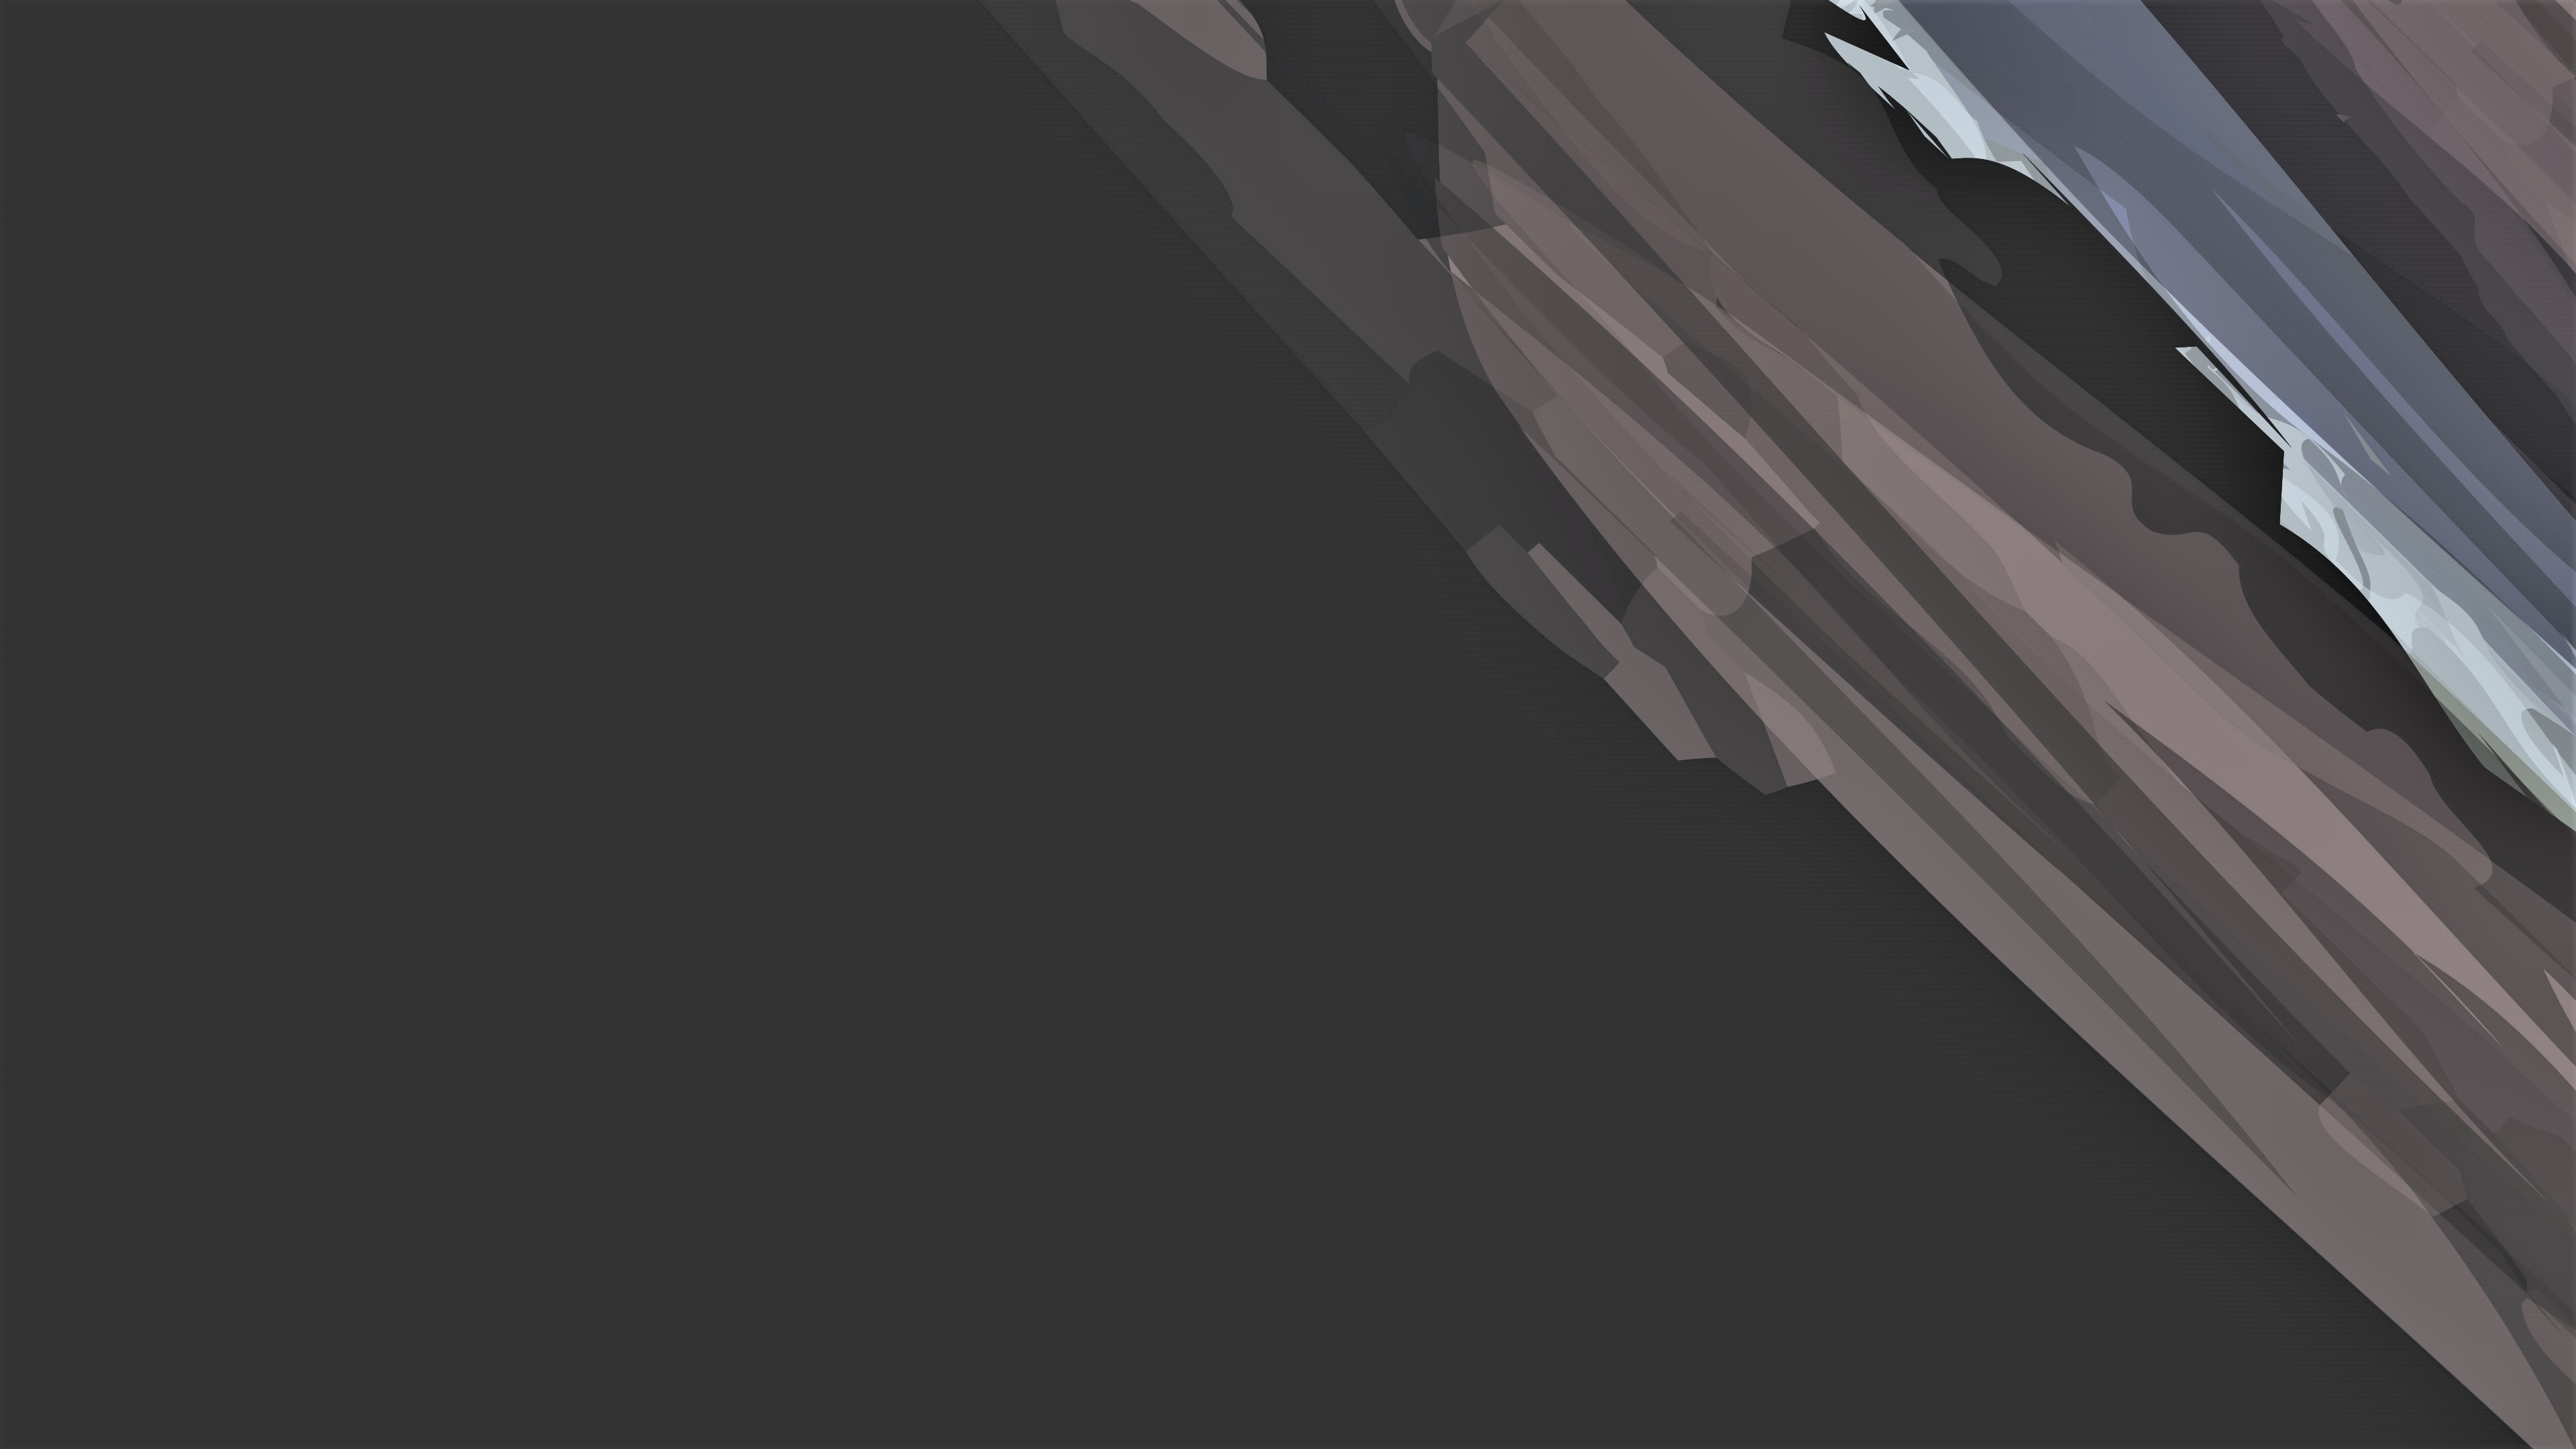
\includegraphics[width=\paperwidth,height=\paperheight]{static/bg}
}
% \setbeamercolor{background canvas}{bg=NavyBlue!50!DarkOliveGreen, fg=white}
\setbeamercolor{normal text}{fg=white}
\maketitle
}%This is the colour of the first slide. bg= background and fg=foreground

\metroset{titleformat frame=smallcaps} %This changes the titles for small caps

% \begin{frame}{Outline}
%   \setbeamertemplate{section in toc}[sections numbered] %This is numbering the sections
%   \tableofcontents[hideallsubsections] %You can comment this line if you want to show the subsections in the table of contents
% \end{frame}

\begin{frame}{Outline}

\begin{itemize}
    \pause
    \item ...
\end{itemize}

\end{frame}


\section{Introduction}
\begin{frame}{Title} 
\begin{itemize}
    \pause
    \item Differential operators are local - they are defined at points.
    \pause
    \item For $d$ a suitable first order derivative, the Lagrangian density with $\phi:(X,g_X)\to(M,g_M)$,
    $$
    L = \|d \phi(x)\|^2_{g_M} d\text{vol}_{g_X}
    $$ 
    is associated to local dynamics \pause \emph{regardless of quantization}.
    \pause
    \item Pseudo-differential operators are generalized derivatives defined on $\Omega\subseteq X$ via an integration rule over $\Omega$ \COMMENT{They do not satisfy Leibniz}
\end{itemize}
\end{frame}

\begin{frame}
    \metroset{block=fill}
    \begin{exampleblock}{\textsc{Def}}
    \begin{equation*}
    (-\Delta)^s f(x) = C_{n,s}\text{p.v.}\int_{\Omega}\frac{f(x)-f(\zeta)}{|x-\zeta|^{n+2s}}d\zeta.
\end{equation*}
or
$$
\mathcal F[(-\Delta)^s](\eta) = |\eta|^{2s}
$$
\end{exampleblock}
\pause
    $$
    L_\gamma = \|(-\Delta)^{\frac{\gamma}{2}} \phi(x)\|^2_{g_M} d\text{vol}_{g_X}
    $$ 
leads to classically nonlocal dynamics \COMMENT{knowing the field configuration at a point and the action does not determine the motion.}
\pause 
\begin{itemize}
    \item Let's call this \emph{classical nonlocality} 
\end{itemize}
\end{frame}


% \end{frame}

\appendix

%% BACKUP %%
\begin{frame}
    Where did the coefficients come from?
    \begin{itemize}
     
        \pause
        \item Define the fractional integration:
        $$
        I^\gamma f(z)=\frac{1}{\Gamma(\gamma)}\int_0^z (z-\zeta)^{\gamma-1}f(\zeta)d\zeta
        $$
        \pause which has the semi-group property $I^{\alpha}I^{\beta}=I^{\alpha+\beta}$.
        \pause
        \item One can then show
        $$
        I^{\gamma} z^{\kappa} = \frac{\Gamma(1+\kappa)}{\Gamma(1+\gamma+\kappa)} z^{\gamma+\kappa}
        $$
        \pause
        \item Now, look at $\partial^\gamma z^{\kappa}=\partial I^{1-\gamma} z^{\kappa}$
        \begin{align*}
        \partial_z ^\gamma z^\kappa &= (\kappa-\gamma+1)\frac{\Gamma(1+\kappa)}{\Gamma(1+1-\gamma+\kappa)}z^{\kappa-\gamma}\\
        &=\frac{\Gamma(1+\kappa)}{\Gamma(1+\kappa-\gamma)}z^{\kappa-\gamma}
        \end{align*}
        \pause
        \item Choosing $\kappa = \gamma k$ gives the desired coefficients - which are now meromorphic functions.
    \end{itemize}
\end{frame}


\end{document}
\underline{\textsc{Some text:}}
\begin{small}
This is some small Text. 
\end{small}

\metroset{block=fill}
\begin{exampleblock}{\textsc{Example block}}
\begin{itemize}
    \item You know how to do itemize
    \item Also here
\end{itemize}
\end{exampleblock}